\documentclass{article}

\usepackage[utf8]{inputenc}
\usepackage{natbib}

\usepackage{graphicx}
\usepackage[section]{placeins}
\usepackage{fullpage}
\usepackage{todonotes}

\usepackage{amsmath}
\usepackage{amssymb}
\usepackage{bbold}
\usepackage{mathrsfs}
\usepackage{bm}

\usepackage{algorithm}
\usepackage[noend]{algorithmic} 

\DeclareMathOperator{\Tr}{Tr}
\DeclareMathOperator{\cst}{cst}
\DeclareMathOperator{\Gram}{Gram}
\DeclareMathOperator{\R}{\mathbb{R}}
\DeclareMathOperator{\1}{\mathbb{1}}
\DeclareMathOperator{\E}{\mathbf{E}}
\DeclareMathOperator{\Y}{\mathcal{Y}}
\DeclareMathOperator*{\argmax}{arg\,max}
\DeclareMathOperator*{\argmin}{arg\,min}
\DeclareMathOperator{\dom}{Dom}

\title{Stochastic Dual Coordinate Ascent \\ for \\ Conditional Random Fields}
\author{R\'emi LE PRIOL}
\date{\today}

\begin{document}

\maketitle

\section*{Introduction}

We apply the Stochastic Dual Coordinate Ascent (SDCA) algorithm to multi-class classification problems.
These problems are formulated as $l^2$ regularized negative log-likelihood minimization. 
We consider their dual : an entropy regularized centroid mean square error.
SDCA update coordinates of the dual variable, one at a time or block by block, so as to raise the dual score.
  
First we focus on problems with a small number of classes for which SDCA's application is straight forward.
This is the framework of multinomial logistic regression.
Then we elaborate the theory for structured prediction problems.
In structured prediction, each class or label is a structured object.
There are too many of these objects to count them all.
More precisely we want to build a map from an input $x$ to a structured output $y$.
$y$ lives in a space that is finite but that is exponentially big in the size of $x$.
However we can use the structure over these $y$ to make the problem tractable.

In Conditional Random Fields (CRF), the labels distribution conditioned on the input is Markov with respect to an undirected graphical model (mathematician language) / Markov random field (computer scientist language). 
The dual problem's natural variables are the joint probabilities over all the potential labels.
We adapt the algorithm to the structure of the output by considering the marginals with respect to the cliques of that graph.

\tableofcontents

\section{Multiclass Logistic Regression}

\subsection{Linear Models}

We consider the following classical supervised setting.
We observe n data points $x_i \in \mathcal{X}$, with their labels $y_i\in \mathcal{Y}:={1,..,K}$, for $i \in {1,..,n}$.
We assume that the pairs $(x_i, y_i)$ are sampled independently and are identically distributed (i.i.d hypothesis).
Given a new vector $x$, we want to predict what is the corresponding label $y$. 
To do so, we first estimate a probability distribution over the classes $p(y|x ; w)$.
$w$ are the \textbf{w}eights that parametrize this distribution. 
The predicted label is then defined as the mode of this distribution : $\hat y = h_w(x) := \argmax_y p(y| x ; w)$.

\paragraph{Features.}
We have no assumption on the space $\mathcal{X}$ but we assume a feature extractor $F:\mathcal{X}\times \mathcal{Y} \rightarrow \R^d$.
These features can be either pre-trained or handcrafted.
For each couple data point - label, we get features as a vector of dimension d.

\paragraph{Linear Assumption.}
The logarithm of our probability can be written as linear function of these features, up to a normalization constant.
The weights vector w has the same dimension as the features.
\begin{equation}
	\label{primal probability}
	p(y | x ; w) := \frac{\exp(w^TF(x, y))}{\sum_{y' \in \mathcal{Y}} \exp(w^TF(x, y'))}
\end{equation}

In the simpler setting, when there is few classes ($K \leq \sim 10^3$), the features we use are a block encoding of the class.
If x are vectors of dimension $d'$, we set $d=Kd'$. $F(x, y=k)$ then has a copy of x on its $k$-th block of size $d'$, and zeros everywhere else.
In terms of linear model, this is the same as having one weights vector $w_k$ per class.
For the sake of comparison, this is like a shallow neural network with no hidden layer.
The input layer is of size $d'$.
The output layer of size K.
The weight matrix W of size $K \times d'$ is the vertical concatenation of the $w_k$.
We apply a softmax on the output layer.

It should be noted that in general $d'$ includes a bias dimension.
The last coordinate of each x is set to 1 (or another constant).
The effective dimension where the x lives is $d'-1$.
With such models, we get polygonal classification boundaries in the space $\mathcal X = \R^{d'}$.
This is shown in figure \ref{linear classification} for $d'=3$.
Only the plan $z=1$ is plotted. In the full 3d space, the decision areas are conic shapes centred on the origin.

\begin{figure}[ht]
	\label{linear classification}
	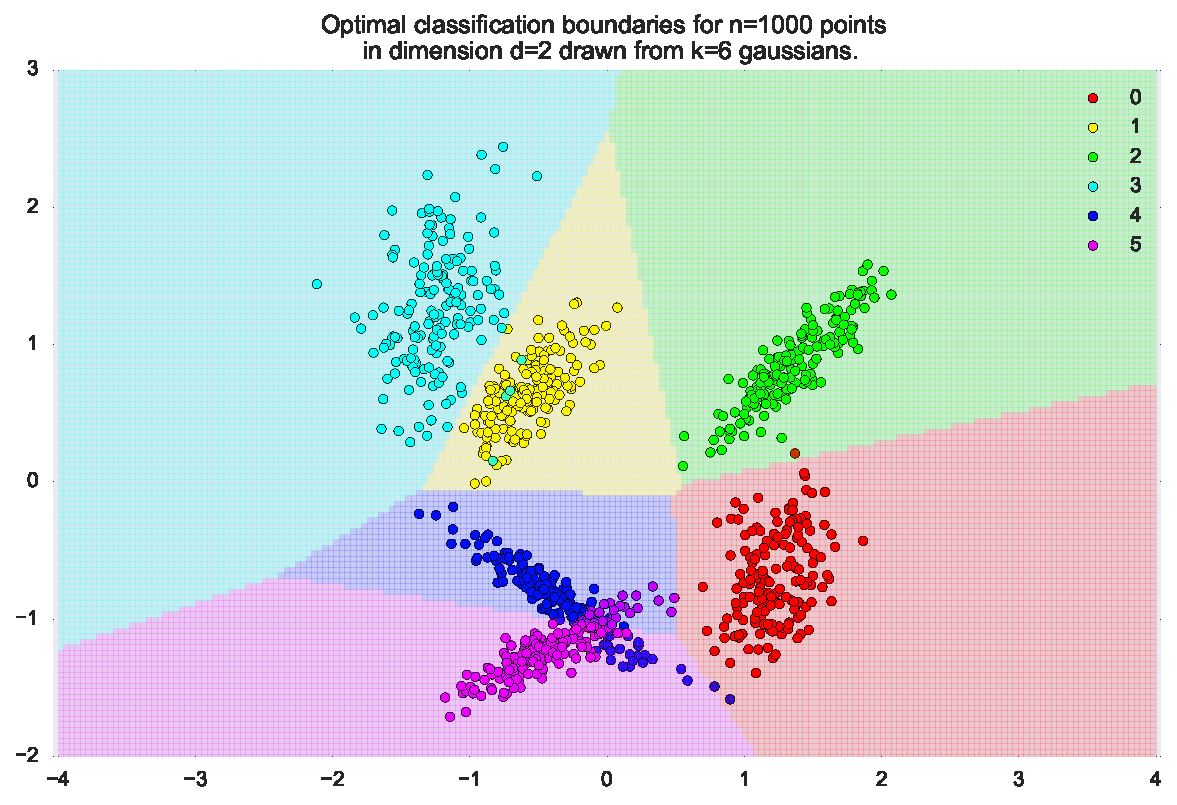
\includegraphics[width=\textwidth]{images/linear_classification.pdf}
	\caption{
	Optimal decision areas for the multinomial logistic regression.
	The data points are drawn from a balanced gaussian mixture in dimension 2.
	We set the bias constant to 1.
	Areas are coloured by the prediction given by a linear model fitted on these points. 
	}
\end{figure}



 \subsection{Maximum Likelihood}

We want to fit our linear model to the observed samples $(x_i, y_i)$.
This means minimizing an empirical loss:
\begin{equation}
	\min_w \sum_{y=1}^K \mathcal L (h_w(x_i),y_i)
\end{equation}
where $\mathcal L: \mathcal Y \times \mathcal Y \rightarrow \R_+$ is a loss between labels.
A typical example is the 0-1 loss $\mathcal L(y, y') : = \1_{y=y'}$.
Unfortunately, this problem is very hard.
Since the loss is defined on a discrete space, there is no notion of continuity, even less so differentiability.
We are left with exhaustive search approaches which are intractable.
Hence the choice to consider the distribution probability $p( . | x ; w) \in \Delta_K$, where $\Delta_K$ denotes the simplex of dimension K.
We replace the discrete space $\mathcal Y$ by the continuous space $\Delta_K$.
We can define continuous or differentiable functions over this space, and get a tractable optimization problem.
 
We want our model to give the maximum probability to the observed pairs $(x_i, y_i)$.
The weights vector maximizing this probability is called maximum likelihood estimator.
Using the independence of the samples, and going to the log space, we formulate this as a sum of negative log-likelihood minimization problem.
To avoid overfitting, we regularize the problem by penalizing the $l^2$ norm of the weights.
We note $\lambda$ the regularization parameter. The primal objective to minimize is:
\begin{equation*}
\mathscr P(w) = \frac{\lambda}{2}\|w\|^2 - \frac{1}{n}   \sum_{i=1}^{n} \log(p(y_i|x_i; w))	
\end{equation*}
Using the linear assumption, we expand the log-likelihood:
\begin{equation*}
	\min_{w\in\R^d} \frac{\lambda}{2}\|w\|^2 + \frac{1}{n}   \sum_{i=1}^{n}  \log \big (\sum_y e^{w^TF(x_i, y)} \big ) - w^TF(x_i, y_i)	
\end{equation*}
To write this in a more compact way, we define the corrected features $\psi_i(y)$ of a class y for the point i as the difference between the ground truth features and the features of $(x_i, y)$.
\begin{equation*}
	\psi_i(y)) := F(x_i, y_i) - F(x_i, y)
\end{equation*}
We can then remove the linear term from the objective:
\begin{equation*}
	\min_{w\in\R^d} \frac{\lambda}{2}\|w\|^2 + \frac{1}{n}   \sum_{i=1}^{n}  \log \big (\sum_y e^{- w^T\psi_i(y)} \big )
\end{equation*}
We can write this problem in a more vectorial form.
Denote the log-partition function (the log-sum-exp) $\phi(z) = \log \big(\sum_{y=1}^K \exp(z_y)\big)$. 
Denote $A_i$ the $d \times |\Y|$ matrix whose columns are the $\psi_i(y)$ for $y \in \Y$.
From now on we will refer to the following formulation as \textit{primal problem}.
\begin{equation}
	\label{primal problem}
	\min_{w\in\R^d}  \frac{\lambda}{2}\|w\|^2 + \frac{1}{n}   \sum_{i=1}^{n} \phi_i(-A_i^Tw)
\end{equation} 

\paragraph{Convexity.}
Let's convince ourselves that this is a convex problem in w.
The $l^2$ penalty is of course convex.
The log-sum-exp is a convex function.
One can verify that it's Hessian is a semi-definite positive matrix -- it is also $1/2$-smooth.
We apply this convex function to a linear transformation over w.
Hence the convexity.
The $l^2$ regularization guarantees that the function we are optimizing is at least $\lambda$ strongly convex. 


\paragraph{Gradients.}
Let's notice that the gradient of the log-partition function evaluated in $-A_i^Tw$ is the conditional probability vector of the classes given x, as defined by the softmax function.
\begin{equation}
	\nabla \phi_i(-A_i^Tw) = (p(y | x ; w))_{y \in \Y}
\end{equation}
The gradient of the right hand term with respect to w is the opposite of the expectation of the corrected features according to these probabilities.
\begin{equation}
	\label{primal gradient}
	\nabla_w (\phi_i(-A_i^Tw)) = - \E_{y \sim p(. | x ; w)} [\psi_i(y)]
\end{equation}
This will prove useful in the following.



\subsection{Dual Formulation}

As any convex problem, the logistic regression admits dual formulations.
In this case, as the problem is unconstrained, we use Fenchel duality theorem to get a dual formulation.

\subsubsection{Derivation}

We write $g(w) :=  \frac{\lambda}{2}\|w\|^2$ the convex regularization function. The primal problem becomes:
\begin{equation*}
	\min_{w \in \R^d}  g(w) + \frac{1}{n} \sum_{i=1}^n \phi_i(- A_i^T w)
\end{equation*}
We note $g^*$ and $\phi_i^*$ the convex conjugates (aka Fenchel dual functions) of $g$ and $\phi_i$ respectively.
The Fenchel dual associated to this problem is derived as follows :
\begin{align*}
	 \min_w \ f(w) + \frac{1}{n} \sum_i \phi_i(- A_i^T w) & = \min_w \ \max_{z\in \dom g^*} z^Tw - g^*(z) + \frac{1}{n} \sum_i \max_{\alpha_i \in \dom \phi_i^*} \alpha_i^T (-A_i^T w) - \phi_i^*(\alpha_i) \\
	 	& \geq \max_{z, \bm \alpha} \  \min_w w^T(z - \frac{1}{n} \sum_i A_i \alpha_i) - g^*(z) - \frac{1}{n} \sum_i \phi_i^*(\alpha_i) \\
		& =  \max_{\bm \alpha} \   - g^*(\frac{1}{n} \sum_i A_i \alpha_i) + \frac{1}{n} \sum_i -\phi_i^*(\alpha_i) \quad \textrm{if} \quad z= \frac{1}{n} \sum_i A_i^T \alpha_i \quad , -\infty \textrm{ otherwise.}\\
\end{align*}
When $g$ is the $l^2$ regularization, the convex conjugate is $g^*: z \mapsto \frac{1}{2\lambda}\|z\|^2$, with domain $\R^d$.
The convex conjugate of the log-sum-exp is the negative entropy. 
Its domain is $\Delta_{|\Y|}$ the simplex of dimension $|\Y|$.
\begin{equation}
	-\phi_i^*(\alpha_i) = H_i(\alpha_i) := - \sum_{y \in \Y} \alpha_i(y) \log(\alpha_i(y))
\end{equation}
Finally we get the canonical dual formulation for the maximum likelihood:
\begin{equation}
	\max_{\bm \alpha | \forall i, \alpha_i \in \Delta_{|\Y|}} \mathscr{D}(\bm \alpha) = -\frac{1}{2\lambda} \| \frac{1}{n} \sum_i A_i^T \alpha_i \|^2 + \frac{1}{n} \sum_{i=1}^n H_i(\alpha_i)
\end{equation}
$\bm \alpha$ is a n*K matrix whose lines live in the simplex.
$\alpha$ should be interpreted as a probability density on the labels for each data point.

\subsubsection{Optimality Condition}
For this problem, \textbf{strong duality holds}.
\begin{verbatim}
https://en.wikipedia.org/wiki/Fenchel%27s_duality_theorem
\end{verbatim} 
\todo { What are the conditions for this. 
In wikipedia, they only talk about the two functions situation.
How is the proof?}

We look at the global optimums $(w^*,z^*,\bm\alpha^*)$.
$(w^*,z^*)$ should be dual variables for the convex conjugates $(g,g^*)$.
\begin{equation*}
	g(w^*) + g^*(z^*) - \langle w^*, z^* \rangle = \frac{\lambda}{2} \| w^* - \frac{1}{\lambda} z^* \|^2 = 0
\end{equation*}
Hence the optimality condition:
\begin{equation*}
	w^* = 	\frac{1}{\lambda} z^* =  \frac{1}{\lambda n} \sum_i A_i^T \alpha_i^*
\end{equation*}
Consequently, we define the dual weights, or primal parameter associated to $\bm \alpha$, with the equation :
\begin{equation}
	\label{dual to primal}
	w(\bm \alpha) =   \frac{1}{\lambda n} \sum_i A_i^T \alpha_i
\end{equation}
The dual problem becomes:
\begin{equation}
	\label{dual problem}
	\max_{\bm \alpha | \forall i, \alpha_i \in \Delta_{|\Y|}} -\frac{\lambda}{2} \| w(\bm \alpha) \|^2 + \frac{1}{n} \sum_{i=1}^n H_i(\alpha_i)
\end{equation}

Formula \ref{dual to primal} can be written in a number of ways, each time outlining some property.
We write A the horizontal concatenation of the $A_i$.
It is a matrix of size $d \times n|\Y|$.
\begin{align}
	w(\bm \alpha) & = \frac{1}{\lambda n} A \alpha \label{linearity} \\
	 & = \frac{1}{\lambda} \E_{i} [ \E_{y \sim \alpha_i} [\psi_i(y)]] \label{corrected features centroid} \\
	 & =   \frac{1}{\lambda} \E_{i} [F(x_i, y_i)] - \frac{1}{\lambda} \E_{i} [ \E_{y \sim \alpha_i} [F(x_i, y)]]
	 \label{centroid difference}
\end{align}
The expectations over i assume that i is a uniform random variable taking its values between 1 and n. 
Equation \ref{linearity} highlights the linearity in $\bm \alpha$. Equation \ref{corrected features centroid} shows that this the centroid of the corrected features. Equation \ref{centroid difference} shows that this is the difference between the empirical feature centroid, and the centroids defined by $\bm \alpha$.

We can also derive the primal problem from the dual problem.
We then get another optimality condition $\bm \alpha(w^*) = \bm \alpha^*$ where $\alpha(w)$ is the probability density on the training set defined by the weights w (equation \ref{primal probability}).
\begin{equation}
	\label{primal to dual}
	\forall i, \alpha_i(w) = \nabla\phi_i(-A_i^Tw) = p(.|x; w) \propto \exp(-w^T \psi_i(.))
\end{equation}

\subsubsection{Interpretation}
The primal problem is a regularized maximization of the likelihood of w. 
In the dual problem \ref{dual problem}, we control directly the probabilities given to each class on the training samples.
There are two conflicting terms.
The left hand one is the opposite of the squared distance between the centroid of the ground truth features and the centroids predicted by the dual model. It is maximal for the empirical distribution.
The second term aims at maximizing the entropy of this distribution.
It pushes the $\alpha_i$ towards a more uniform distribution.
Thus the role of the terms is inverted compared to the primal problem : the data fitting term is the squared euclidean distance, and the regularization is the entropy.

\paragraph{Naming :} 
We call \textit{primal model}, the one where we are given \textit{primal weights} $w$, from which we deduce \textit{primal probabilities} $\alpha_i(w)$.
We call \textit{dual model}, the one where we are given \textit{dual probabilities} $\alpha_i$, from which we deduce \textit{dual weights} $w(\alpha)$ as the centroid of the corrected feature vectors.
The optimality conditions tell us that at the optimum, these two models are equal.
They weights are the centroid of the corrected features, and the dual probabilities are given by the softmax function.


%%%%%%%%%%%%%
\subsection{Duality Gaps}

The duality gap $g(w,\alpha)$ is the difference between the value  of the primal problem evaluated in $w$, and the value of the dual problem evaluated in $\alpha$.
\begin{equation*}
	g(w,\bm \alpha) := \mathscr P(w) - \mathscr D(\bm \alpha)
\end{equation*}
It is interesting to look at the duality gap for both the primal model and the dual model, i.e. the duality gap between the primal weights and the primal probability, and the duality gap between the dual weights and the dual probability.

\paragraph{Primal model:}
We inject the expression of $\alpha_i(w)$ in the entropy to find the formula:
\begin{equation}
	\label{primal duality gap}
	g(w,\bm \alpha(w)) = \frac{\lambda}{2} \|w-w(\alpha(w))\|^2
\end{equation}
This formula involves $w(\alpha(w))$.
This is what the dual model created by the primal probabilities think the weights should be. 

In fact, using equation \ref{primal gradient} and \ref{dual to primal}, we can express the gradient of the primal objective 	as :
\begin{align*}
	\nabla \mathscr P(w) 
	& = \lambda w + \frac{1}{n} \sum_i \nabla_w(\phi_i(-A_i^Tw)) \\
	& = \lambda \bigg [ w - \frac{1}{\lambda n} \sum_i \E_{y \sim p(. | x ; w)} [\psi_i(y)] \bigg ] \\
	& = \lambda [ w - w(\bm \alpha(w))]
\end{align*}
This means that the squared norm of the batch gradient is proportional to a duality gap.
\begin{equation}
	g(w,\bm \alpha(w)) = \frac{1}{2 \lambda} \|\nabla \mathscr P(w)\|^2
\end{equation}
In SAG, (see \cite{schmidt_non-uniform_2015}), Marc Schmidt et al. use an estimate of the gradient of the former as a descent direction.
They also use the norm of this estimate as a certificate to decide when to stop.
The justification was that the gradient converges toward zero.
If the objective is m-strongly convex there is also the bound:
\begin{equation*}
	\mathscr P (w) - \mathscr P(w^*) \leq \frac{1}{2 m}\|\nabla \mathscr P (w)\|^2
\end{equation*}
since the objective is at least $\lambda$-strongly convex we retrieve that the duality gap dominates the primal sub-optimality.

\paragraph{Dual model:}
The gap for the dual model is naturally expressed as a sum of Fenchel duality gaps between the convex conjugates $\phi_i$ and $-H_i$. 
\begin{align*}
	g(w(\bm \alpha),\bm \alpha) 
	& = \frac{1}{n} \sum_i \big [ \phi_i(-A_i^Tw(\bm \alpha)) - H_i(\alpha_i) \big ] + \lambda \|w(\bm \alpha)\|^2 \\
	& =  \frac{1}{n} \sum_i \big [ \phi_i(-A_i^Tw(\bm \alpha)) - H_i(\alpha_i) - \langle \alpha_i,  -A_I^T w(\bm \alpha) \rangle \big ]
\end{align*}
Each of the divergence in the sum above is of course positive.
They can be thought of as the duality gaps associated to each data point for the dual model.
In particular, we have $\log(\alpha_i(w)) = -A_i^Tw - \phi_i(-A_i^Tw) \1$. Since $\alpha_i$ sums to one, we can inject this expression in the scalar product. We then get that each of the Fenchel duality gaps is also equal to the Kullback-Leibler divergence between the dual probability and the primal probability defined by the dual weights $w(\bm \alpha)$.
\begin{equation}
	\label{dual duality gaps}
	g(w(\bm \alpha),\bm \alpha) = \frac{1}{n} \sum_i D_{KL} (\alpha_i || \alpha_i(w(\alpha))
\end{equation}
Once again, we observe a loop. Starting from the dual model, we define a primal which in turn defines a dual model.
\textit{Remark:} Performing SDCA with a step-size $\gamma=1$ gives the update formula $\alpha_i^+ = \alpha_i(w(\alpha))$, i.e. $ D(\alpha_i^+ || \alpha_i(w(\alpha)) )=0$. (See next section).

%%%%%%%%%%%%%%%%%
\subsection{Stochastic Dual Coordinate Ascent}
The SDCA algorithm updates the dual variable, one coordinate at a time, so as to maximize the dual objective $\mathscr D(\bm \alpha)$.
In our case, the dual probabilities $\alpha_i$ are constrained to live in the simplex.
We have to update the variables one block at a time.
The most natural way is to update one probability vector $\alpha_i \in \Delta_K$ altogether.
This is what Shalev-Schwartz studied in his articles \cite{shalev-shwartz_accelerated_2013-1}.
Finding the optimal update for $\alpha_i$ is a constrained optimization problem in dimension K, which is itself difficult. 
The brilliant idea analyzed by Shalev-Shwartz is to update $\alpha_i$ towards a sub-gradient of the primal loss $\nabla\phi_i( - A_i^Tw(\alpha)) = \alpha_i(w(\bm \alpha))$.
This way, $\alpha_i$ is getting closer from what it should be equal to $\alpha_i(w(\bm \alpha)$, and we can guarantee that the duality gap decreases enough.
Plus, since $\Delta_K$ is convex, we are guaranteed to stay within the simplex after each step.  
Formally, we define the dual ascent direction and the associated primal descent direction:
\begin{align*}
	d_i &:= \alpha_i(w(\alpha)) - \alpha_i \\
	v_i &:= \frac{1}{\lambda n} A_i d_i  = \frac{1}{\lambda n} \big [ \E_{y \sim \alpha_i} [F(x_i, y)] - \E_{y \sim  \alpha_i(w(\alpha))} [F(x_i, y)] \big ]
\end{align*} 
The update formula is:
\begin{equation*}
	\alpha_i^+ \leftarrow \alpha_i + \gamma d_i = (1-\gamma)\alpha_i + \gamma \alpha_i(w(\bm \alpha)) \quad \textrm{with} \quad \gamma \in [0,1]
\end{equation*}
The step size $\gamma$ is either fixed, either found via a line search on the segment between $\alpha_i$ and $\alpha_i(w(\alpha))$. 
It belongs in $[0,1]$ because we want a convex combination of $\alpha_i$ and $\alpha_i(w(\alpha))$ to remain in the simplex without further checks. 
Most importantly, it is necessary for the proof of the linear convergence rate in \cite{shalev-shwartz_accelerated_2013-1}. 
See algorithm \ref{sdca for logreg} for details.


\begin{algorithm}[ht]
    \caption{SDCA for Logistic Regression}%
    \label{sdca for logreg}
\begin{algorithmic}
        %
        \STATE $\forall i,$ initialize $\alpha_i^{(0)}$ at random in $\Delta_K$
        \STATE Let $w^{(0)} = \frac{1}{\lambda n} A \bm \alpha$  
        \STATE Let $\forall i,\  g_i = 1$ (optional)
        %
       \FOR{$k=0\dots K$}
                \STATE Pick $i$ at random in $\{1,\ldots,n\}$ (optionally, proportional to $g_i$)
                \STATE Let $ \beta_i := p( . |x ; w^{(k)})$
                %
                \STATE Let $g_i = D_{KL}(\alpha_i || \beta_i)$ (optional)
                %
                \STATE Let $d_i = \beta_i - \alpha_i^{(k)}$ (dual ascent direction)
                \STATE Let $v_i = \frac{1}{\lambda n} A_i d_i $ (primal descent direction)
                \STATE Solve $\gamma^* = \argmax_{\gamma \in [0,1]} H_i(\alpha_i^{(k)} + \gamma d_i) - \frac{\lambda n}{2} \| w^{(k)} + \gamma v_i \|^2$ (Line Search)
                %
               \STATE Update $\alpha_i^{(k+1)} := \alpha_i^{(k)} + \gamma^* d_i$
               \STATE Update $w^{(k+1)} := w^{(k)} + \gamma^* v_i $
        \ENDFOR
\end{algorithmic}
\end{algorithm}


\paragraph{Line search:} 
the function of the step size we want to maximize is 
\begin{equation}
	\label{line search 1}
	f_i(\gamma) = -\frac{\lambda n}{2} \|w + \gamma v_i\|^2 + H(\alpha_i + \gamma d_i) + \cst
\end{equation}
where $d_{[i]}$ is the matrix n*K whose line i is $d_i$ and where the rest is 0.
We expand the first term in equation \ref{line search 1} with the formulation above to highlight the quadratic dependency on $\gamma$.
Calculating the derivatives is straight forward.
\begin{align*}
	f(\gamma)
	& = H_i(\alpha_i^{(k)} + \gamma d_i)
	- \gamma \lambda n  \langle w^{(k)} , v_i \rangle 
	- \gamma^2 \frac{\lambda n}{2} \|v_i \|^2
	+ \cst
	\\
	f'(\gamma) & =  - \langle d_i, \log(\alpha_i + \gamma d_i) \rangle
	- \lambda n \langle w^{(k)} , v_i \rangle 
	- \gamma \lambda n \|v_i \|^2 
	\\
	f''(\gamma) & = - \sum_{y} \frac{d_{i}(y)^2 }{ \alpha_i(y) + \gamma d_i(y) }
	- \lambda n  \|v_i \|^2 
\end{align*}
We compute $\langle w^{(k)} , v_i \rangle$ and $ \|v_i \|^2$ once and for all at the beginning of each line search for a cost $O(d)$. Then each function estimate has a toll $O(\|Y\|)$.\\
We can find the $2\epsilon$-approximate maximum of $f'$ defined on ]0,1[ by looking at its $\epsilon$-approximate root on $[\epsilon,1-\epsilon]$.
This can be done with a stabilized Newton method for instance, as described in the section 9-4 of the book \cite{press_numerical_1992}.

\paragraph{Non-Uniform Sampling:} 
In the article \cite{osokin_minding_2016}, the authors improve the empirical rate of convergence of their stochastic algorithm with non-uniform sampling.
More precisely, they sample data points with a probability proportional to past-estimates of the individual duality gaps.
They can apply this scheme because the algorithm Block Coordinate Frank-Wolfe \cite{lacoste-julien_block-coordinate_2012} gives an individual duality gap for free at each time step.
To make this work, they have to perform a batch update of their duality gaps every ten epochs or so.

In SDCA, we have access to duality gap $g_i$ if we pick the element i for almost no extra cost.
Each step involves computing $\alpha_i(W(\alpha))=\nabla\phi(s_i)$.
Computing the KL-divergence takes a complexity $O(K)$.

\subsection{Results}

SDCA gives proper results on synthetic gaussian mixtures datasets. 
\begin{figure}[ht]
	\label{gmm results}
	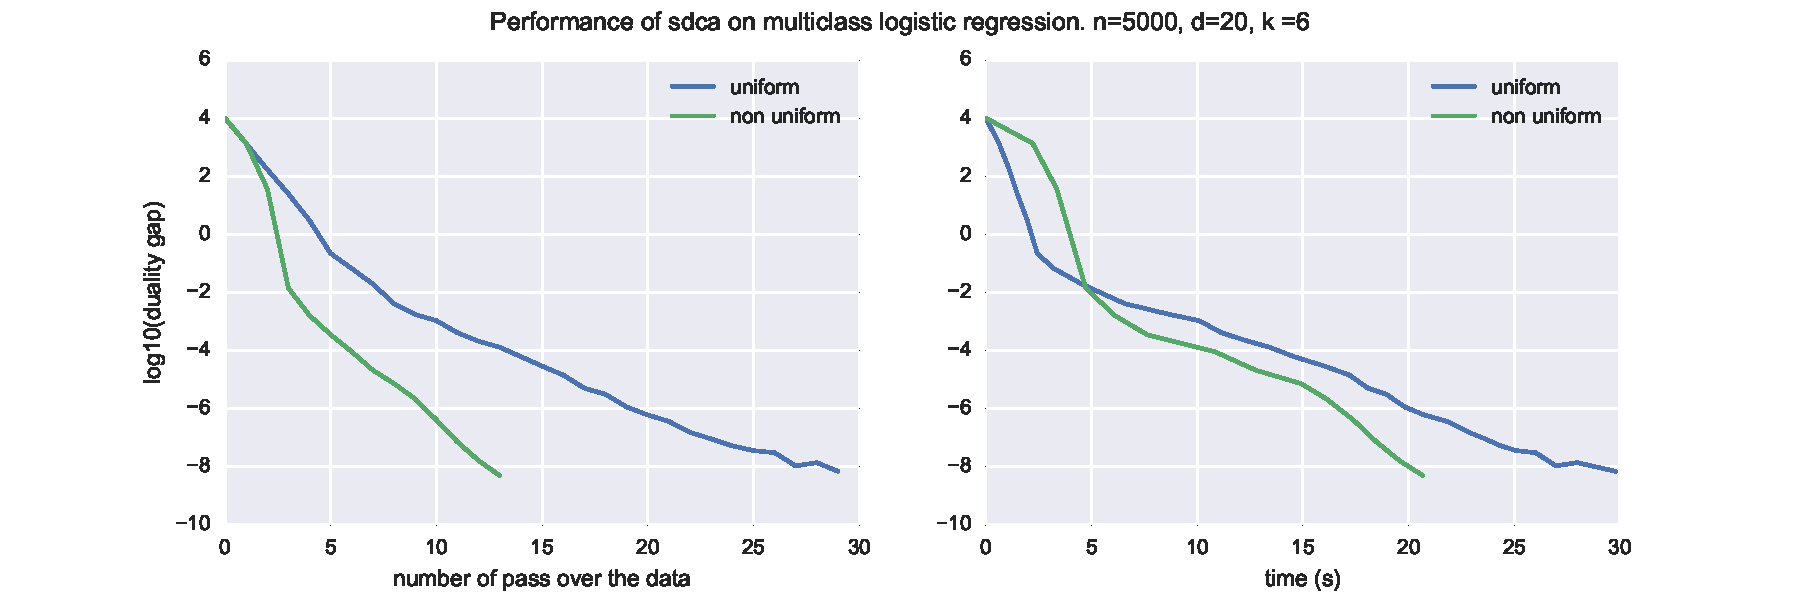
\includegraphics[width=\textwidth]{images/nonuniform_is_better.pdf}
	\caption{Comparison of the performance of various methods on a synthetic Gaussian mixture dataset.}
\end{figure}

\todo{Comparison with the other non-uniform sampling method on a real dataset?}


%%%%%%%%%%%%%%%%%%%%%%%%%%%%%%%%%%%%%%%%%%%%%%%%%%%%%%%%
% CRF 
%%%%%%%%%%%%%%%%%%%%%%%%%%%%%%%%%%%%%%%%%%%%%%%%%%%%%%%%
\clearpage
\section{Conditional Random Fields}

\subsection{Structured Prediction}

Structured prediction is a category of multi-class classification problems.
The particularity is that we have information about the structure of the classes.
For instance we would like to identify a word of length T from T images of letters, and we know that there is a chain structure on these letters (OCR \todo{put citation   here}).
Or we could parse sentences and we know that there is a natural tree structure defined by the grammar.
Another typical instance is semantic segmentation in images : we know a priori that boundaries between objects should be sharp and that objects are usually connected areas.
Let's write x for the input data point and y for the output class that lives in $\Y_x$.
We index $x$ to $\Y$ because the space of classes can depend on $x$.
For instance, the word we predict will have as many letters as we have images, and the semantic segmentation will be an image of the same size as the input image. 

Compared to standard multi-class classification, we need to exploit the structure because the output space $\Y_x$ has a size that is typically exponential in the size of the input x.
Even for prediction, a brute force approach listing the probabilities class by class and taking the max is intractable.
The structure generally allows us to explore the space of classes in a clever way, to compute the mode of this distribution or the marginal probabilities on some part of the structure.
We call the algorithm that returns the mode the \textit{max oracle} and the one that returns the marginals the \textit{marginalization oracle}.
They are black boxes for the optimization algorithm, hence the name oracle.
They generally take time.
The performance of a structured prediction algorithm is generally measured by the number of oracle calls.
In reality, marginalization oracle are often slower than maximization oracle, and there are a number of operations besides these oracles.
Yet the number of oracle call gives a good idea of the overall complexity of an algorithm.

Formally, for any pair (input, output) we want to define a structured score $s_w(x, y)$ parametrized by a vector w.
This score should represent the confidence that we have that the point x belongs to the class y through the equation $p(y|x ; w)\propto \exp(s_w(x, y))$.
Physically, the score  is thus the opposite of the energy of the state y for the system x. 
\begin{equation}
	p(y|x; w)=  \frac{e^{s_w(x, y)}}{\sum_{y'} e^{s_w(x, y')}}
\end{equation}

In the following, we assume that we have a feature extractor for pairs $x, y \mapsto F(x, y) \in \R^d$, either handcrafted or pre-trained.
Our score will be a linear combination of these features.
We call the parameter w \textit{the weights}.
\begin{equation}
	s_w(x, y) = \langle w, F(x, y) \rangle
\end{equation}

We consider output spaces specified by undirected graphical models, aka Markov Random Fields.
The output y is a random variable that factors over the graph $G=(V,E)$.
Formally, this means that the joint probability over y can be factorized into potentials over the maximal cliques of the graph.
We denote the $\mathcal{C}$ the set of maximal cliques of G, and $\mathcal{S}$ the set of separations between these cliques.

\begin{align*}
	p(y|x ; w) & \propto  \exp(s_w(x, y) \\
	& \propto \prod_{c\in \mathcal{C}} \exp(s_{w, c}(x, y_c))\\
	& \propto  \prod_{c\in \mathcal{C}} \exp(\langle w, F_c(x, y_c) \rangle) \\
	& \propto \exp( \langle w, \sum_{c\in \mathcal{C}} F_c(x, y_c) \rangle 
\end{align*}
We go from the second to the third line by assuming that the score of each clique is itself linear.
The consequence of these derivations is that if y factors over a graph, we want the features to be separable the same way :
\begin{equation}
	F(x, y) =  \sum_{c\in \mathcal{C}} F_c(x, y_c)
\end{equation}


\subsection{Maximum Likelihood}

We have a set of n pairs $(x_i, y_i) \in \mathcal{X} \times \Y_i$ independently sampled.
We also have a feature extractor that maps these pairs to $\R^d$.
This feature extractor is separable over graphs of the appropriate dimension corresponding to each $\Y_i$.
The Conditional Random Field model aims at maximizing the log-likelihood of the weights $w\in \R^d$ given these samples.
Once we have learnt the weights, we can predict the class of a new data point x by taking the mode of $p(y|x ; w)$.
The prediction function is thus $x \mapsto \hat{y} = h_w(x) = \argmax_{y\in \Y_x} s_w(x, y)$.
To avoid overfitting and to make the problem strongly convex, we penalize the squared $l^2$ norm of the weights.
The variational CRF problem is written below.

\begin{equation}
\min_{w\in\R^d} f(w) = \frac{\lambda}{2}\|w\|^2 - \frac{1}{n}   \sum_{i=1}^{n} \log(p(y_i|x_i; w))	
\end{equation}

Let's expand the probability term in this formula.
We define the corrected features $\psi_i(y)$ of a class y for the point i as the difference between the ground truth features and the features of $(x_i, y)$.
\begin{equation}
	\psi_i(y)) := F(x_i, y_i) - F(x_i, y)
\end{equation}
The negative log-likelihood then becomes the log-partition function (log-sum-exp) $\phi_i(z):=\log(\sum_{y\in \Y_i} e^{z(y)})$ over these features.
\begin{equation}
	- \log(p(y_i|x_i; w)) = \log \bigg ( \sum_{y \in \Y_i}  \exp(-w^T\psi_i(y)) \bigg ) = \phi_i(-A_i^Tw)	
\end{equation}
where $A_i$ \todo{Change the name of $A_i$ for a more typical one.
Idem for $\phi_i$} is the $d\times |\Y_i|$ matrix whose columns are the $\psi_i(y)$ for $y \in \Y_i$.
We index $i$ to $\phi_i$ because it affects the range of the sum.
The closed formulation of the CRF is thus :

\begin{equation}
\min_{w\in\R^d} f(w) = \frac{\lambda}{2}\|w\|^2 + \frac{1}{n}   \sum_{i=1}^{n} \phi_i(-A_i^Tw)	
\end{equation}


%%%%%%%%%%%%%%%%%%%%%%%%%%%%%%%%%%%%%%%%%%%%%%%%%%%%%%%%%%
\subsection{Dual Formulation}

We can derive a Fenchel dual to the CRF, as done in \todo{provide reference.}
\begin{equation}
	\max_{\alpha\in\Delta_{1} \times \dots \times \Delta_{n}} -\frac{\lambda}{2}\|w(\alpha)\| +\frac{1}{n} \sum_{i=1}^n H_i(\alpha_i)
\end{equation}
where $\Delta_i$ is the simplex of dimension $|\Y_i|$, meaning that $\alpha$ is a n*$|\Y_i|$ matrix whose lines live in the simplex, and $H_i$ is the entropy for distributions over $\Y_i$ : $H(\alpha_i) := - \sum_y \alpha_i(y) \log(\alpha_i(y)$.
To simplify the notation, we omit the domain of summation for y in the sum as it can be deduced from the context.
We define the \textit{dual weights} given by the optimality condition:
\begin{equation*}
	w(\alpha) = \frac{1}{\lambda n} \sum_i \sum_y \alpha_i(y) \psi_i(y) 
\end{equation*}
At the dual optimum $\alpha^*$, $w(\alpha^*)$ is optimum for the primal problem.
This formula can be written in a number of ways, each time outlining some property.
\begin{align}
	w(\alpha) & = \frac{1}{\lambda n} A \alpha \label{linear combination of probabilities} \\
	 & = \frac{1}{\lambda} \E_{i} [ \E_{y \sim \alpha_i} [\psi_i(y)]] \label{mean of the corrected features} \\
	 & =   \frac{1}{\lambda} \E_{i} [F(x_i, y_i)] - \frac{1}{\lambda} \E_{i} [ \E_{y \sim \alpha_i} [F(x_i, y)]]
	 \label{difference between ground truth and dual weights}
\end{align}
where A is the horizontal concatenation of the $A_i$.
It is a matrix of size $d \times \sum_i |\Y_i|$.
The expectations over i assume i is uniform random variable taking its values between 1 and n. 

\paragraph{Interpretation :} The primal problem is a regularized maximization of the likelihood of w. 
In the dual problem, we control directly the probabilities given to each class on the training samples.
There is two conflicting terms.
The first one aims at minimizing the size of the centroid of the corrected features.
Since $\psi_i(y_i)=0$, it is minimal for the empirical distribution.
The second term aims at maximizing the entropy of this distribution.
It pushes the $\alpha_i$ towards a more uniform distribution.
Thus the role of the terms is the inverse of the primal model : the data fitting term is on the left.
It is the squared distance between the centroid of the ground truth features and the centroids predicted by the dual model.
The entropy on the right is the regularization. 

We can also derive the primal problem from the dual problem.
We then get another optimality condition $\alpha(w^*) = \alpha*$ where $\alpha(w)$ is the density on the training set defined by the weights w in equation \ref{primal probability}.

\begin{equation}
	\forall i, \alpha_i(w) = \nabla\phi_i(-A_i^Tw) = p(.|x; w) \propto \exp(-w^T \psi_i(.))
\end{equation}

\paragraph{Naming :} 
We call \textit{primal model}, the one where we are given \textit{primal weights} w, from which we deduce \textit{primal probabilities} $\alpha_i(w)$.
We call \textit{dual model}, the one where we are given \textit{dual probabilities} $\alpha_i$, from which we deduce \textit{dual weights} $w(\alpha)$ as the centroid of the corrected feature vectors.
The optimality conditions tell us that at the optimum, these two models are equal.

%%%%%%%%%%%%%%%%%%%%%%%%%%%%%%%%%%%%%%%%%%%%%%%%%%%%%%%%
\subsection{Marginalization}

Taking the raw dual problem is intractable.
The variable $\alpha$ itself is a priori too big to fit in memory : for each data point, it stores a probability vector that is exponential in the size of this data point.
This is where the structure comes into play.
We assume that the output class y factors over a triangulated Markov random field $G=(V,E)$ with a junction tree $T=(\mathcal{C},\mathcal{S})$.
Then the joint probability $\alpha(y)$ can be written as a function of its marginals $\mu$.
We keep the notation $\mathcal{C}$ for the set of maximal cliques of G, and $\mathcal{S}$ the set of separations between these cliques along a junction tree.
The marginal over a set of nodes $s$, is given by $\mu_s(y_s) = \sum_{y' | y_s'=y_s} \alpha(y)$. 
\begin{equation}
	\label{joint from marginals}
	\alpha(y) = \frac{\prod_{c\in\mathcal{C}} \mu_c(y_c)}{\prod_{s\in\mathcal{S}} \mu_s(y_s)}
\end{equation}

$\mu$ should be thought of as the marginals over the cliques only.
The $\mu_s$ are a byproduct of these.
When we go from the joint $\alpha_i$ to the marginal $\mu_i$, we go from a size $\Y_i$, to a size $\sum_{c \in \mathcal C_i} |\Y_c|$.
If each component of y can take K values, then we go from $K^{|V_i|}$ to $\sum_{c \in \mathcal C_i} K^{|c|}$ which should be considerably smaller.
The formula \ref{joint from marginals} make sense as long as the marginals on the maximal cliques are coherent, meaning that they agree about the values of the marginals on the separations.
Our algorithm will make sure that this coherence is preserved at each step.
\ref{joint from marginals} allows us to translate each of the functions previously seen with the joint, in functions of the marginals.
First the entropy and the Kullback-Leibler divergence.

\begin{equation}
	H_{|\Y|} (\alpha) = \sum_c H_{|c|}(\mu_c) - \sum_s H_{|s|}(\mu_s) =: \mathcal H (\mu) 
	\label{marginals entropy}
\end{equation}
\begin{equation}
	D(\alpha||\alpha') = \sum_c D(\mu_c||\mu_c') - \sum_s D(\mu_s||\mu_s') =: \mathcal D (\mu||\mu')
\end{equation}

We can also write the dual weights as a function of the marginals :

\begin{align*}
	   \E_{\alpha_i}[\psi_i]
   & = \sum_{y \in \Y_i} \alpha_i(y) \psi_i(y)  \\
   &  = \sum_{c \in \mathcal C_i} \sum_{y \in \Y_i}  \alpha_i(y)  \psi_{i, c}(y_c)  \\
   & = \sum_{c \in \mathcal C_i}\sum_{y_c \in  \Y_c} \bigg ( \sum_{y'| y'_c = y_c } \alpha_i(y') \bigg ) \psi_{i, c}(y_c) \\
   & = \sum_{c \in \mathcal C_i}\sum_{y_c \in \Y_c} \mu_{i, c}(y_c)  \psi_{i, c}(y)
\end{align*}

As we have done with $w(\alpha)$, we can reformulate this.
Let  $B_i$ be the matrix of size $d \times  \sum_{c \in \mathcal C_i} |\Y_c|$, whose columns are the $\psi_{i, c}(y)$.
Let $B$ be the horizontal concatenation of the $B_i$.
Let $\mu$ be the vector containing all the $\mu_i$.

\begin{align}
	w (\mu)
	& =\frac{1}{\lambda n} \sum_i \sum_{c \in \mathcal C_i} \E_{\mu_i}[\psi_{i, c}] \\
	& = \frac{1}{\lambda} B\mu \label{marginals to primal}
\end{align}

With equations \ref{marginals entropy} and \ref{marginals to primal} we can write the dual problem as a maximization over the marginals.
\begin{equation}
	\max_{\forall i \forall c, \mu_{i, c} \in \Delta_{|c|} } - \frac{\lambda}{2} \|w(\mu)\|^2 + \frac{1}{n} \sum_i \mathcal H _ i(\mu)
\end{equation}

\subsection{SDCA}

As we have seen in the introduction about structured prediction, the separation of the feature vectors is equivalent to the factorisation of the primal probabilities.
We can get the primal marginals with a marginalization oracle, such as message passing on a junction tree. 

\begin{algorithm}[ht]
    \caption{SDCA for CRF}%
    \label{sdca for crf}
\begin{algorithmic}
        %
        \STATE Let $\forall i, c, \mu_{i, c}^{(0)} := \frac{1}{|c|}$ and $w^{(0)} := \frac{1}{\lambda n} B \mu^{(0)} $
        \STATE Let $\forall i g_i = 1$ (optional)
        %
       \FOR{$k=0\dots K$}
                \STATE Pick $i$ at random in $\{1,\ldots,n\}$ (optionally, proportional to $g_i$)
                \STATE Compute $\forall c, \mu_{i, c}' (y_c) := p(y_c|x; w^{(k)})$ (marginalization oracle)
                %
                \STATE Let $g_i = \mathcal D(\mu_i || \mu_i')$ (optional)
                %
                \STATE Let $d_i = \mu_i' - \mu_i^{(k)}$ (ascent direction)
                \STATE Let $v_i = \frac{1}{\lambda} B_i d_i $ (primal direction)
                \STATE Solve $\gamma^* = \argmax_{\gamma \in [0,1]} \mathcal H_i(\mu_i^{(k)} + \gamma d_i) - \frac{\lambda n}{2} \| w^{(k)} + \frac{\gamma}{n} v_i \|^2$ (Line Search)
                %
               \STATE Update $\mu_i^{(k+1)} := \mu_i^{(k)} + \gamma^* d_i$
               \STATE Update $w^{(k+1)} := w^{(k)} + \frac{\gamma^*}{n} v_i $
        \ENDFOR
\end{algorithmic}
\end{algorithm}

\paragraph{Complexity:} ascent direction in $O(\sum_c |\Y_c|)$ and primal direction in $O(d*\sum_c |\Y_c|)$.
The line search is not too expensive.
Each function or gradient evaluation is $O(\sum_c |\Y_c|)$.

Note that the computation of $w^{(0)}$ can usually be hand made very efficiently.

Every T pass, do a full pas over the data to compute the true duality gap, which gives a stopping criterion.

\paragraph{Line Search:} we optimize over $\gamma \in [0,1]$ because we want a convex combination of $\mu_i$ and $\nabla_i$.
It gives us a guarantee that we stay in the simplex without any further checks.
Plus $\gamma$ a priori has no incentives to be outside of $[0,1]$, since $\mu_i$ and $\nabla_i$ are converging towards each other.
The marginals over the separation $\mu_{i, s}$ and $d_{i, s}$ are computed once and for all at the beginning of the line search.

\begin{align*}
	f(\gamma)
	& = \mathcal H_i(\mu_i^{(k)} + \gamma d_i) 
	- \frac{\lambda n}{2} \| w^{(k)} + \frac{\gamma}{n} v_i \|^2 
	\\
	& =  \sum_c H_{|c|}(\mu_c + \gamma d_{i, c}) 
	- \sum_s H_{|s|}(\mu_s + \gamma d_{i, s}) 
	- \frac{\lambda n}{2} \| w^{(k)}\|^2 
	- \gamma \lambda  \langle w^{(k)} , v_i \rangle 
	- \gamma^2 \frac{\lambda}{2n} \|v_i \|^2 
	\\
	f'(\gamma) & =  - \sum_c \langle d_{i, c}, \log(\mu_c + \gamma d_{i, c}) \rangle 
	+ \sum_s \langle d_{i, s} , \log(\mu_s + \gamma d_{i, s}) \rangle 
	- \lambda  \langle w^{(k)} , v_i \rangle 
	- \gamma \frac{\lambda}{n} \|v_i \|^2 
	\\
	f''(\gamma) & = - \sum_c \sum_{y_c} \frac{d_{i, c}(y_c)^2 }{ \mu_c(y_c) + \gamma d_{i, c}(y_c) }
	+ \sum_s \sum_{y_s} \frac{d_{i, s}(y_s)^2 }{ \mu_s(y_s) + \gamma d_{i, s}(y_s) }
	- \frac{\lambda}{n} \|v_i \|^2 
\end{align*}


\bibliographystyle{plain}
\bibliography{optimization.bib}

\end{document}